\documentclass[a4paper]{article}

\usepackage[french]{babel}
\usepackage[utf8]{inputenc}
\usepackage[T1]{fontenc}
\usepackage{fullpage}
\usepackage{hyperref}
\usepackage{graphicx}
\usepackage{float}
\usepackage{amsmath}
\usepackage{amssymb}
\usepackage{color}
\usepackage{listings}

\lstset{
  language=SQL,
  basicstyle=\ttfamily\footnotesize,        % the size of the fonts that are used for the code
  breakatwhitespace=false,         % sets if automatic breaks should only happen at whitespace
  breaklines=true,                 % sets automatic line breaking
  commentstyle=\color{cyan},    % comment style
  keepspaces=true,                 % keeps spaces in text, useful for keeping indentation of code (possibly needs columns=flexible)
  keywordstyle=\color{blue},       % keyword style
  numbers=left,                    % where to put the line-numbers; possible values are (none, left, right)
  numbersep=5pt,                   % how far the line-numbers are from the code
  numberstyle=\tiny\color{blue}, % the style that is used for the line-numbers
  rulecolor=\color{black},         % if not set, the frame-color may be changed on line-breaks within not-black text (e.g. comments (green here))
  showstringspaces=false,          % underline spaces within strings only
  showtabs=false,                  % show tabs within strings adding particular underscores
  stepnumber=5,                    % the step between two line-numbers. If it's 1, each line will be numbered
  stringstyle=\color{red},     % string literal style
  tabsize=2,                       % sets default tabsize to 2 spaces
}

\author{Titouan \bsc{Christophe}\\Florentin \bsc{Hennecker}\\Rodrigue \bsc{Van Brande}}
\title{Synthèse de bases de données}
\date{\today}

\begin{document}
\maketitle
\tableofcontents

\section{Modèle entité-association}
Un schéma conceptuel des données, pas forcément implémenté de cette façon.
Selon le contexte, désigne la classe (modèle) ou l'objet (l'instance).

\paragraph{Remarque} Le nom \textbf{Entité-Relation} est équivalent à
\textbf{Entité-Relationel} ou encore \textbf{Entité-Association}

\subsection{Entité}
\begin{figure}[H]
    \center
    \includegraphics[width=.3\textwidth]{fig/entity.png}
    \caption{Une entité}
\end{figure}

\subsubsection{Attributs}
Les entités ont des attributs, qui ont une cardinalité minimale et maximale

\paragraph{Attributs multivalués}
Attributs dont la cardinalité maximale est supérieure à 1.
Exemple: \texttt{Person.degrees}

\paragraph{Attributs dérivés}
Attributs calculés à partir d'autres attributs, pas stockés dans la base de donnée.
Exemple: à partir du champ \texttt{Person.birth}, on peu déduire \texttt{Person.age}

\paragraph{Attributs composites}
Attributs formés par l'aggrégation de plusieurs autres attributs.
Exemple: \texttt{Person.Adress = \{Street, City, State, Zipcode, Country\}}

\paragraph{Clefs ou identificateurs}
Attributs ou ensemble d'attributs d'une entité dont les valeurs sont uniques
(déterminent une et une seule entité). On les met en évidence dans un schéma
entité-association en les soulignant, en ajoutant un symbole \textit{clef} à côté,
ou en les mettant dans une section à part dans la boîte de l'entité.
\subparagraph{Clefs primaires}
Seule l'une des clefs peut être soulignée, et est l'identifiant d'un objet pour
cette entité.

\subsection{Association}
\begin{figure}[H]
    \center
    \includegraphics[width=.4\textwidth]{fig/relation.png}
    \caption{\label{fig:relation}Une relation One-to-many}
\end{figure}
\begin{figure}[H]
    \center
    \includegraphics[width=.3\textwidth]{fig/relation-ensembliste.png}
    \caption{Vue ensembliste de la relation à la Figure \ref{fig:relation}}
\end{figure}
\begin{itemize}
  \item On doit spécifier la multiplicité minimale et maximale pour chaque pair de la relation
  \item La relation porte un nom (souvent lié au sens et à la sémantique de la relation)
  \item Chaque entité à un rôle dans la relation
  \item Une relation peut contenir des attributs
  \item L'arité ($x$-ary) d'une relation, ou son \textbf{degré}, indique le nombre d'entités participant à la relation
  \item \textbf{One-to-one}, \textbf{one-to-many} ou \textbf{many-to-many} pour les relations binaires
\end{itemize}

On peut noter qu'il n'y a pas de différence fondamentale entre un attribut et une relation,
juste une question de point de vue. On préfèrera une relation si on souhaite mettre en évidence
les liens entre plusieurs objets, et un attribut quand c'est une propriété comme un autre.

\subsubsection{Relation n-aire}
Une relation n-aire implique plus que 2 entités différentes.

\begin{figure}[H]
    \center
    \includegraphics[width=.4\textwidth]{fig/relation-naire.png}
    \caption{Une relation ternaire et sa vue ensembliste}
\end{figure}

\subsubsection{Transformation des relation n-aires en binaires}
Les relations obtenues après transformation \textbf{par projection} contiennent moins d'information
que la relation initiale. Par exemple, dans la Figure \ref{fig:relation-naire-projection},
on voit que la relation ternaire indique qu'un fournisseur délivre un produit pour un projet,
tandis que les relations binaires indiquent uniquement qu'un fournisseur délivre un produit,
qu'un projet utilise un produit, et qu'un projet utilise un fournisseur.

\paragraph{Projection}
On crée une relation pour chaque paire possible de la relation
\begin{figure}[H]
    \center
    \includegraphics[width=.4\textwidth]{fig/relation-naire-projection.png}
    \caption{\label{fig:relation-naire-projection}Projection d'une relation ternaire}
\end{figure}

\paragraph{Insertion}
On transforme la relation en entité, et on la lie par des relations binaires à
toutes les entités de la relation initiale.
\begin{figure}[H]
    \center
    \includegraphics[width=.6\textwidth]{fig/relation-naire-insertion.png}
    \caption{Transformation par insertion}
\end{figure}

\subsection{Entités faibles}
Une entité faible n'a aucune clef ne dépendant que de ses propres attributs, et
a donc une \textbf{clef partielle} qui la distingue des autres entités ayant la
même clef étrangère.

\paragraph{Intérêt des entités faibles}
\begin{itemize}
  \item Suppression des attributs redondants
  \item Réduction des relation n-aires en relations binaires par la méthode d'insertion
  \item Héritage et polymorphisme (ajout des attributs des entités filles dans des entités faibles)
\end{itemize}

\subsection{Relation génériques}
\'Equivalent des design pattern pour les relations. Elle dénotent la nature d'une
relation sur un schéma entité-association.

\subsubsection{Classification}
Utilisée lorsqu'on instancie un objet. Exemple: on a une liste de destinations
au départ d'un aéroport (classe), et les vols chaque jour vers ces destinations (instance).

\subsubsection{Généralisation (héritage)}
Relation spéciale entre une ou plusieurs sous-entités et une superentité, plus abstraite.

\begin{figure}[H]
    \center
    \includegraphics[width=.3\textwidth]{fig/generalisation.png}
    \caption{Généralisation}
\end{figure}

\paragraph{Différent types de recouvrements}
\begin{itemize}
  \item \textbf{Partiel} ou \textbf{Total}: les entité filles ont-elles des attributs de la superentité ?
  \item \textbf{Exclusif} ou \textbf{Recouvrant (overlapping)}: les entités filles partagent-elles des attributs ?
  \item La spécialisation peut être déterminée par un prédicat (ex: \texttt{Person.age < 18 -> Child})
  \item Les clefs sont héritées, et de nouvelles clefs peuvent être définies par les entités filles
\end{itemize}
\begin{figure}[H]
    \center
    \includegraphics[width=.6\textwidth]{fig/generalisation-cov.png}
    \caption{Combinaisons de recouvrements partiels et totaux, exclusifs et recouvrants}
\end{figure}

Les contraintes de recouvrement influencent l'implémentation.


%%%%%%%%%%%%%%%%%%%%%%%%%%%%%%%%%%%%%%%%%%%%%%%%%%%%%%%

\section{Modèle relationnel}
Données structurées en tables bidimensionnels de valeurs simples. Les lignes
sont aussi appelées tuples, et les colonnes attributs.
Les relations sont des tables avec des restrictions:
\begin{itemize}
  \item L'ordre des lignes n'a pas d'importance
  \item L'ordre des colonnes n'a pas d'importance
  \item La table a au moins une clef (pas de lignes en double exemplaire)
\end{itemize}
La relation peut être vue comme un prédicat, par exemple comme un ensemble de propriétés.

Les bases de données sont des collections de relations, mais ne pas oublier que
les structures relationnelles sont plus riches que les tables, et que le modèle de 
données ne définit pas que les structures de données, mais aussi des opérations
pour les manipuler.

\subsection{Schéma}
On parle du schéma pour décrire le modèle des données (le nom des colonnes).

\begin{figure}[H]
    \center
    \includegraphics[width=.5\textwidth]{fig/relmodel-er.png}
    \caption{\label{fig:relmodel-er}Un modèle entité-association}
\end{figure}
\begin{figure}[H]
    \center
    \includegraphics[width=.7\textwidth]{fig/relmodel-tuples.png}
    \caption{Les tuples correspondant au schéma Figure \ref{fig:relmodel-er}}
\end{figure}

Lors de la traduction du modèle entité-association en modèle relationnel, on voit
que toutes les relations ne sont pas matérialisées par une table (par exemple,
un \texttt{Department} contient directement la clef de son manager et sa date d'entrée en service),
et que certaines tables ne sont pas modélisées par une entité ou une relation, mais
par un attribut multivalué (\texttt{Department.location})

\subsection{Relations}
Le schéma auquel on adjoint les valeurs donnent une relation. Plus formellement, on a
\begin{equation}
  R(A_1:D_1, ~ ... ~ , A_n:D_n)
\end{equation}
Où $R$ est la relation, les $D_i$ sont un ensemble de valeurs atomiques appelées le \textbf{domaine},
les attributs $A_i$ sont distincts dans la relation. $A_i : D_i$ dénote la structure de la relation.
\'Etant donné un tuple\footnote{un ensemble de paires attribut:valeur} $\{A_1: d_1, ~...~, A_n: d_n\}$, on a la valeur relationelle
\begin{equation}
  \rho \subseteq \{\{A_1:d_1, ~...~, A_n:d_n\} \mid d_i \in D_i\}
\end{equation}

Le domaine définit la comparabilité des valeurs: des attributs ne peuvent être comparés
que s'ils sont sur le même domaine. On peut voir le domaine comme des types définis par
l'utilisateur.

\subsection{Clefs de relation}

\paragraph{Une super-clef} désigne un ou plusieurs attributs qui, ensemble, identifient
un et un seul tuple.

\paragraph{Une clef} est une super-clef minimale (si un seul des attributs est
enlevé de la super-clef minimale, elle perd sa propriété d'identification unique).
Généralement, une relation a plusieurs clefs, qu'on appelle aussi clefs candidates.

\paragraph{La clef primaire} est une clef choisie parmi les clefs candidates comme étant
la seule qu'on utilisera pour identifier un tuple.

\subsection{Contraintes relationnelles}
Les contraintes font parties du schéma, et spécifient des prescriptions ou
assertions sur les données. Elles permettent de garantir l'intégrité des données.

\subsubsection{Intégrité référentielle}
\'Etant donné une contrainte relationelle sur $R_1$ et $R_2$, $\exists$ un attribut
$A_2$ de $R_2$ tq. $A_2$ a le même domaine que la clef primaire de $R_1$ et toute
valeur de $A_2$ dans un tuple de $R_2$ apparaît comme clef primaire dans le tuple
de $R_1$. On appelle $A_2$ une clef étrangère. $A_2$ n'est pas forcément une clef
de $R_2$

\begin{figure}[H]
    \center
    \includegraphics[width=.7\textwidth]{fig/integrite-rel.png}
    \caption{Intégrité référentielle du schéma Figure \ref{fig:relmodel-er}}
\end{figure}

\subsubsection{Contraintes transitionelles}
On impose une contrainte sur la mise à jour de la valeur d'un attribut (exemple:
une personne ne peut pas changer de sexe, un salaire ne peut qu'augmenter...)

\subsubsection{Contraintes structurelles}
\paragraph{Intégrité de la clef}
Toute relation a une clef primaire et éventuellement d'autres clefs

\paragraph{Intégrité de domaine}
Les valeurs des attributs doivent correspondre au domaine (type et opérations permises)

\paragraph{Intégrité de l'entité}
Les clefs primaires ne sont pas nulles

\paragraph{Intégrité de colonne}
Une contrainte spécifique imposée sur une colonne (ex: la date est supérieure à l'an 2000)

\paragraph{Intégrité de ligne}
Contrainte sur un tuple en particulier (ex: la date de retraite doit être postérieure
à la date de premier emploi).

\subsubsection{Suppression d'un tuple}
Quand la suppression d'un tuple viole une contrainte d'intégrité référentielle,
il faut exécuter une des actions suivantes :
\begin{itemize}
  \item rejeter la suppression
  \item propager la suppression aux tuples qui référencent le tuple supprimé
  \item nullifier les valeurs d'attributs des tuples qui référencent le tuple supprimé,
  sauf si ces attributs font partie de la clé primaire
\end{itemize}

\subsection{Implémentation dans les DBMS}
Un DBMS a donc:
\paragraph{Un langage de définition des données (DDL)} permettant de créer le schéma
\paragraph{Un langage de manipulation des données (DML)} pour accéder aux valeurs.
Par exemple, l'algèbre relationelle ou le calcul tuple. SQM redéfinit les opérations
correspondantes et définit quelques extensions (les fonctions d'aggrégation par exemple).
\paragraph{Des opération d'altération} permettant de modifier ou supprimer des valeurs et des schémas.
Ces opérations doivent tenir compte des contraintes (en émettant une erreur si l'une d'elle est violée par exemple).
\paragraph{Des vues (éventuellement)} décrivant des relations dérivées
(relations inférées à partir d'autres). Elles peuvent être enregistrées sur le
disque (snapshots), mais ça peut poser des problème de redondance.

\subsection{Traduction depuis un schéma E-R}
\subsubsection{Suppression des généralisations}
\paragraph{Tout dans la superentité}
Tous les champs de toutes les entités filles sont dans la superentité. Les attributs
inexistants pour une entité fille sont nuls. On rajoute un champ pour déterminer
le type d'enfant du tuple (dans l'exemple ci-dessous, \texttt{Rank}).\\

Il faut parfois également rajouter des contraintes (ci-dessous, par exemple :
seulement les étudiants avec \texttt{Rank == GradStud} ont un advisor).
\subparagraph{Avantage}
Facile et rapide à mettre en place, toujours utilisable.
\subparagraph{Inconvénients}
Gaspillage d'espace (beaucoup d'attributs nuls), les opérations sur les entités
filles doivent être exprimée sur la superentit (programme plus complexe).
\begin{figure}[H]
    \center
    \includegraphics[width=.7\textwidth]{fig/er2rm-1.png}
\end{figure}

\paragraph{Garder les entités filles}
On ne crée que les entités feuilles dans l'arbre d'héritage, il n'existe pas de
table pour la superentité. Chaque entité fille contient ses attributs propres et
ceux de sa superentité. \textbf{Il faut garantir avec une contrainte que les
clefs sont uniques parmis l'ensemble de toutes les entités filles.}
\subparagraph{Inconvénients}
Beaucoup d'attribut redondants et de relations, rendant les applications plus complexes.
Utilisable avec les relations totales-exclusives uniquement.
\begin{figure}[H]
    \center
    \includegraphics[width=.9\textwidth]{fig/er2rm-2.png}
\end{figure}

\paragraph{Transformation en relations}
Une table pour chaque entité. On crée une relation one-to-one entre une entité
et sa superentité. Les filles sont des entités faibles.
\subparagraph{Inconvénients}
Redondance (beaucoup de relations signifient la même chose), il faut des contraintes
pour exprimer le type de généralisation (recouvrement). Les opération deviennent plus
complexes (en O(n) de la profondeur de l'arbre d'héritage).
\begin{figure}[H]
    \center
    \includegraphics[width=.9\textwidth]{fig/er2rm-3.png}
\end{figure}

\subsubsection{Règles de traduction}
\paragraph{Entités}
Pour toutes les entités non-faibles $E$ créer une relation $R$ qui a tous les attributs
de $E$. On identifie les clefs, et les attributs composites sont stocké champ par champ.

\paragraph{Entité faibles}
Création d'une relation $R$ pour chaque entité faible $E$, contenant tous ses
attributs simples, et les clefs des entités référencées comme clefs étrangères.

\paragraph{Relation one-to-one}
Choisir une des deux entité comme faible, et y insérer une clef étrangère qui
est la clef primaire de l'autre.

\paragraph{Relation one-to-many}
L'entité du côté many est transformée en une relation $R$ possèdant une clef étrangère
qui référence la clef primaire de l'autre relation

\paragraph{Relation many-to-many}
On crée une relation pour chaque entité, et une relation avec une clef étrangère
qui référencent les deux autres relations (on passe de 2 à 3 tables).

\paragraph{Attributs multivalués}
\subparagraph{Avec une relation supplémentaire}
On traduit une entité $E$ contenant un attribut multivalué en relation $R$.
On crée une relation contenant une clef étrangère vers la clef primaire de $R$ et
une des valeurs de l'attribut.
\begin{figure}[H]
    \center
    \includegraphics[width=.7\textwidth]{fig/multiattrs-1nf.png}
    \caption{Transformation des attributs multivalués en ajoutant une relation}
\end{figure}

\subparagraph{Avec une seule relation}
On ajoute une ligne par valeur de l'attribut multivalué pour un même objet.
\begin{figure}[H]
    \center
    \includegraphics[width=.7\textwidth]{fig/multiattrs-single.png}
    \caption{Transformation des attributs multivalués en une seule relation}
\end{figure}

\subsubsection{Perte d'information}
La traduction amène à une perte de précision: une relation (dans le modèle relationnel)
peut traduire plusieurs entités et relations du modèle E-R. Une bonne correspondance
entre les deux modèle nécessite des bonnes contraintes d'intégrité et référentielles,
ainsi qu'une documentation mettant le modèle E-R en relation avec la structure relationelle.


%%%%%%%%%%%%%%%%%%%%%%%%%%%%%%%%%%%%%%%%%%%%%%%%%%

\section{Algèbre relationnel}

L'algèbre relationnel est un ensemble d'opérateurs qui agissent sur une ou plusieurs
relations et qui produisent une relation en sortie.

  \subsection{Sélection (ou restriction)}
  On ne prend que les tuples qui satisfont une (ou plusieurs) condition(s).

    $$ \sigma_{condition}(R) = \{r\in R\, |\, condition(r)\} $$

  Intuition : la sélection est une tranche horizontale d'une relation.
  
  Exemple:
  \begin{tabular}{|c|c|c|}
	\multicolumn{3}{c}{R}\\
	\hline
	A & B & C\\
	\hline\hline
	1 & a & 1\\
	2 & a & 1\\
	3 & c & 2\\
	4 & d & 2\\
	\hline
  \end{tabular}
  $\rightarrow \sigma_{C=2}(R) \rightarrow$
  \begin{tabular}{|c|c|c|}
	\hline
	A & B & C\\
	\hline\hline
	3 & c & 2\\
	4 & d & 2\\
	\hline
  \end{tabular}

  \subsection{Projection}
  Garder seulement un ensemble d'attributs d'une relation.

  $$ \pi_{attributs}(R) $$

  Intuition : la projection est une tranche verticale d'une relation.

    Exemple:
  \begin{tabular}{|c|c|c|}
	\multicolumn{3}{c}{R}\\
	\hline
	A & B & C\\
	\hline\hline
	1 & a & 1\\
	2 & a & 1\\
	3 & c & 2\\
	4 & d & 2\\
	\hline
  \end{tabular}
  $\rightarrow \pi_{B,C}(R) \rightarrow$
  \begin{tabular}{|c|c|c|}
	\hline
	B & C\\
	\hline\hline
	a & 1\\
	c & 2\\
	d & 2\\
	\hline
  \end{tabular}
  
  \paragraph{Suppression des doublons}
  La projection fait en plus une suppression des doublons.

  \subsection{Combinaison d'opérations}

  \paragraph{Forme imbriquée} de type $ \pi_{FName, LName}(\sigma_{DNo<3\; \lor\; DNo=5 }(Employee))$

  \paragraph{Forme séquentielle}
  \begin{align*}
    Temp &\leftarrow \sigma_{DNo=5}(Employee)\\
    R(FirstName, LastName) &\leftarrow \pi_{FName, LName}(Temp)
  \end{align*}

  \subsection{Opérations ensemblistes}

  \paragraph{Union} $R \cup S$ : tous les tuples dans R, dans S ou dans R et S (sans doublon)

  \paragraph{Intersection} $R \cap S$ : tous les tuples dans R et dans S

  \paragraph{Différence} $R - S$ : tous les tuples dans R mais pas dans S\\

  Ces opérations ne se font que sur des relations dont les attributs sont
  de même types un à un.
  
  
      Exemple:
\begin{tabular}{|c|c|}
	\multicolumn{2}{c}{Student}\\
	\hline
	FName & LName\\
	\hline\hline
	Susan & Yao\\
	Ramesh & Shah\\
	Barbara & Jones\\
	Amy & Ford\\
	Jimmy & Wang\\
	\hline
\end{tabular}
\begin{tabular}{|c|c|}
	\multicolumn{2}{c}{Prof}\\
	\hline
	FName & LName\\
	\hline\hline
	John & Smith\\
	Ricardo & Brown\\
	Susan  &Yao\\
	Francis  & Johnson\\
	Ramesh & Shah\\
	\hline
\end{tabular}\\
\begin{tabular}{|c|c|}
	\multicolumn{2}{c}{\textcolor[rgb]{1,0,0}{Student $\cup$ Prof}}\\
	\hline
	FName & LName\\
	\hline\hline
	Susan & Yao\\
	Ramesh & Shah\\
	Barbara & Jones\\
	Amy & Ford\\
	Jimmy & Wang\\
	John & Smith\\
	Ricardo & Brown\\
	Francis & Johnson\\
	\hline
\end{tabular}
\begin{tabular}{|c|c|}
	\multicolumn{2}{c}{\textcolor[rgb]{1,0,0}{Student $\cap$ Prof}}\\
	\hline
	FName & LName\\
	\hline\hline
	Susan & Yao\\
	Ramesh & Shah\\
	\hline
\end{tabular}
\begin{tabular}{|c|c|}
	\multicolumn{2}{c}{\textcolor[rgb]{1,0,0}{Student - Prof}}\\
	\hline
	FName & LName\\
	\hline\hline
	Barbara & Jones\\
	Amy & Ford\\
	Jimmy & Wang\\
	\hline
\end{tabular}
	
  

  \subsection{Renommage}
  Dans certains cas (voir produit cartésien), il faut renommer certains attributs
  d'une relation. On le fait de la manière suivante :
  $$ \alpha_{originalAttributeName:newAttributeName}(R) $$
  
  Exemple:
  \begin{tabular}{|c|c|c|}
	\multicolumn{3}{c}{R}\\
	\hline
	A & B & C\\
	\hline\hline
	1 & a & 1\\
	2 & a & 1\\
	3 & c & 2\\
	4 & d & 2\\
	\hline
  \end{tabular}
  $\rightarrow \alpha_{C,D}(R)$ ou $R(A,B,D)\leftarrow R \rightarrow$
  \begin{tabular}{|c|c|c|}
	\hline
	A& B & \textcolor[rgb]{1,0,0}{D}\\
	\hline\hline
	1 & a & 1\\
	2 & a & 1\\
	3 & c & 2\\
	4 & d & 2\\
	\hline
  \end{tabular}

  \subsection{Produit cartésien}
  Le produit cartésien $R \times S$ associe chaque tuple d'une relation avec tous les tuples
  d'une autre relation. Puisque tous les attributs de chaque relation se retrouvent
  dans le résultat, si certains attributs ont les mêmes noms, il faut les renommer.
  
  Exemple:
  \begin{tabular}{|c|c|}
	\multicolumn{2}{c}{R}\\
	\hline
	A & B\\
	\hline\hline
	A1 & B1\\
	A2 & B2\\
	\hline
  \end{tabular}
  \begin{tabular}{|c|c|}
	\multicolumn{2}{c}{S}\\
	\hline
	C & D\\
	\hline\hline
	C1 & D1\\
	C2 & D2\\
	\hline
  \end{tabular}
  \begin{tabular}{|c|c|c|c|}
	\multicolumn{4}{c}{\textcolor[rgb]{1,0,0}{R $\times$ S}}\\
	\hline
	A & B & C & D\\
	\hline\hline
	A1 & B1 & C1 & D1\\
	A1 & B1 & C2 & D2\\
	A2 & B2 & C1 & D1\\
	A2 & B2 & C2 & D2\\
	\hline
  \end{tabular}

  \subsection{Jointure}
  La jointure (aussi appelée jointure $\theta$) n'est en fait qu'un produit cartésien suivi d'une sélection. 
  La condition exprimée sur la jointure est effectivement la condition de la sélection.

  $$R \bowtie_{condition} S = \{concat(r,s)\; |\; r \in R\; \land \; s \in S\; \land \; condition(r,s)\} $$

  N'oublions pas que certains attributs de R ou de S pourraient devoir être renommés.\\

  Les notations des paragraphes suivants proviennent de wikipedia :
  
  Exemple:
  \begin{tabular}{|c|c|}
	\multicolumn{2}{c}{R}\\
	\hline
	A & B\\
	\hline\hline
	a & b\\
	c & b\\
	d & e\\
	\hline
  \end{tabular}
  \begin{tabular}{|c|c|}
	\multicolumn{2}{c}{S}\\
	\hline
	C & D\\
	\hline\hline
	b & c\\
	e & a\\
	b & d\\
	\hline
  \end{tabular}
  \begin{tabular}{|c|c|c|c|}
	\multicolumn{4}{c}{\textcolor[rgb]{1,0,0}{R $\bowtie_{B=C}$ S}}\\
	\hline
	A & B & C & D\\
	\hline\hline
	a & b & b & c\\
	a & b & b & d\\
	c & b & b & c\\
	c & b & b & d\\
	d & e & e & a\\
	\hline
  \end{tabular}

  \paragraph{Jointure naturelle} $R \bowtie S$ : pour tous les attributs qui se trouvent en même temps dans R et dans S, on garde les tuples qui ont les mêmes 
  valeurs pour ces attributs dans R et dans S.
  
    Exemple:
  \begin{tabular}{|c|c|}
	\multicolumn{2}{c}{R}\\
	\hline
	A & B\\
	\hline\hline
	a & b\\
	c & b\\
	d & e\\
	\hline
  \end{tabular}
  \begin{tabular}{|c|c|}
	\multicolumn{2}{c}{S}\\
	\hline
	B & C\\
	\hline\hline
	b & c\\
	e & a\\
	b & d\\
	\hline
  \end{tabular}
  \begin{tabular}{|c|c|c|}
	\multicolumn{3}{c}{\textcolor[rgb]{1,0,0}{R $*$ S}}\\
	\hline
	A & B & C\\
	\hline\hline
	a & b & c\\
	a & b & d\\
	c & b & c\\
	c & b & d\\
	d & e & a\\
	\hline
  \end{tabular}

  \paragraph{Equijoin} $R \bowtie_{A=B} S$ : Jointure $\theta$ avec une seule 
  condition qui est une égalité.\\
  
  
    Exemple:
  \begin{tabular}{|c|c|}
	\multicolumn{2}{c}{R}\\
	\hline
	A & B\\
	\hline\hline
	a & b\\
	c & b\\
	d & e\\
	\hline
  \end{tabular}
  \begin{tabular}{|c|c|}
	\multicolumn{2}{c}{S}\\
	\hline
	C & D\\
	\hline\hline
	b & c\\
	e & a\\
	b & d\\
	\hline
  \end{tabular}
  \begin{tabular}{|c|c|c|c|}
	\multicolumn{4}{c}{\textcolor[rgb]{1,0,0}{$R \bowtie_{B=C} S$}}\\
	\hline
	A & B & C & D\\
	\hline\hline
	a & b & b & c\\
	a & b & b & d\\
	c & b & b & c\\
	c & b & b & d\\
	d & e & e & a\\
	\hline
  \end{tabular}

  \paragraph{Left Outer Join} $\sqsupset\,\bowtie$ : Jointure $\theta$ ou seul les tuples de gauche sans correspondances
  sont gardées (les valeurs pour les attributs de la table de droite sont mise à NULL ($\omega$).\\
  
    Exemple:
  \begin{tabular}{|c|c|}
	\multicolumn{2}{c}{R}\\
	\hline
	A & B\\
	\hline\hline
	a & b\\
	c & b\\
	d & e\\
	\hline
  \end{tabular}
  \begin{tabular}{|c|c|}
	\multicolumn{2}{c}{S}\\
	\hline
	B & C\\
	\hline\hline
	b & c\\
	\hline
  \end{tabular}
  \begin{tabular}{|c|c|c|}
	\multicolumn{3}{c}{\textcolor[rgb]{1,0,0}{$R \sqsupset\, \bowtie S$}}\\
	\hline
	A & B & C\\
	\hline\hline
	a & b & c\\
	c & b & c\\
	d & e & $\omega$\\
	\hline
  \end{tabular}
  
  \paragraph{Right Outer Join} $\bowtie\,\sqsubset$ : Jointure $\theta$ ou seul les tuples de droite sans correspondances
  sont gardées (les valeurs pour les attributs de la table de gauche sont mise à NULL ($\omega$).\\
  
    Exemple:
  \begin{tabular}{|c|c|}
	\multicolumn{2}{c}{R}\\
	\hline
	A & B\\
	\hline\hline
	a & b\\
	c & b\\
	\hline
  \end{tabular}
  \begin{tabular}{|c|c|}
	\multicolumn{2}{c}{S}\\
	\hline
	B & C\\
	\hline\hline
	b & c\\
	e & f\\
	\hline
  \end{tabular}
  \begin{tabular}{|c|c|c|}
	\multicolumn{3}{c}{\textcolor[rgb]{1,0,0}{$R \bowtie\, \sqsubset S$}}\\
	\hline
	A & B & C\\
	\hline\hline
	a & b & c\\
	c & b & c\\
	$\omega$ & e & f\\
	\hline
  \end{tabular}
  \paragraph{Full Outer Join} $\sqsupset\,\bowtie\,\sqsubset$: Jointure $\theta$ combinant le \emph{Left Outer Join} et le \emph{Right Outer Join},
  Toutes les tuples n'ayant pas de correspondance, à gauche, ou à droite, sont aussi retranscrit avec les valeurs NULL ($\omega$) pour les correspondances.
  
    Exemple:
  \begin{tabular}{|c|c|}
	\multicolumn{2}{c}{R}\\
	\hline
	A & B\\
	\hline\hline
	a & b\\
	c & b\\
	c & d\\
	\hline
  \end{tabular}
  \begin{tabular}{|c|c|}
	\multicolumn{2}{c}{S}\\
	\hline
	B & C\\
	\hline\hline
	b & c\\
	e & f\\
	\hline
  \end{tabular}
  \begin{tabular}{|c|c|c|}
	\multicolumn{3}{c}{\textcolor[rgb]{1,0,0}{$R \sqsupset\,\bowtie\,\sqsubset S$}}\\
	\hline
	A & B & C\\
	\hline\hline
	a & b & c\\
	c & b & c\\
	c & d & $\omega$\\
	$\omega$ & e & f\\
	\hline
  \end{tabular}  

  \subsection{Division}
  $$ R(A,B)\; \div\; S(B) $$
  Tous les tuples de $\pi_{A}(R)$ qui apparaissent dans R avec au moins chaque
  élément de S.

  \begin{figure}[H]
    \center
    \includegraphics[width=.25\textwidth]{fig/relalg-division.png}
  \end{figure}

  \subsection{Outer Union}
  Si R et S sont partiellement compatibles, l'outer union garde tous les attributs
  et le annule s'ils ne sont pas applicables pour ce tuple.

%%%%%%%%%%%%%%%%%%%%%%%%%%%%%%%%%%%%%%%%%%%%%%%%%%

\section{Calcul relationnel}
  Cette section traite de la structure logique des Relational Query Languages.
  On utilise la logique du premier ordre.\\

  \subsection{Calcul relationnel tuple}
  La structure générale d'une requête en calcul tuple relationnel est :
  $$ \{t_1.A_1, t_2.A_2,...,t_n.A_n\; | \; F(t_1, ... t_n,t_{n+1},...t_{m})\} $$
  avec :
  \begin{itemize}
    \item $t_1, t_2,...t_m$ les variables tuple associées à $F$ avec une relation
    via un prédicat de relation\footnote{wat}
    \item $A_i$ : les attributs de la relation associée à $t_i$
    \item F : la formule logique qui contient $t_1,...,t_m$
    \item $t_1,...;t_n$ les variables libres de F ("variables de query")
    \item $t_{n+1},...,t_m$ les variables quantifiées dans F
  \end{itemize}

  \subsubsection{Quantificateur existentiel}
  Voici un join (le quantificateur existentiel est généralement utilisé pour les
  join) :
  \begin{align*}
    \{e.Lname, e.Address\; | \; &Employee(e)\\
    &\land\, \exists d (Department(d) \,\land\, d.Manager = 'KrazyBen'\, \land\, d.DNumber = e.DNo)\} )
  \end{align*}

  \subsubsection{Quantificateur universel}
  Le quantificateur universel est très utile pour les divisions.
  Il doit toujours être associé avec l'implication. Pourquoi? Prenons l'exemple
  de cours prérequis. On veut tous les étudiants qui ont passé les prérequis
  de Plasticine. Si on a cette formule : $\forall p (Prereq(p) \land \exists etudiant ...$ et que Plasticine n'a aucun prérequis, la formule renvoie un ensemble
  vide alors que tous les étudiants ont passé les "aucun" prérequis.
  \begin{align*}
    \{e.Lname\; | \; &Employee(e)\\
    &\land\, \forall d (Dependent(d) \,\rightarrow\, e.SSN = d.ESSN)\} )
  \end{align*}

  \subsection{Calcul relationnel domaine}
  La structure générale d'une requête en calcul relationnel domaine est :
  $$ \{x_1, s_2,...,x_n\; | \; F(x_1, ... x_n,x_{n+1},...x_{m})\} $$
  avec $R(A_i:x_i,...A_j:x_j)$.

  \subsubsection{Quantificateur existentiel}
  Voici un exemple simple :
  \begin{align*}
    \{fn, ln\; |\; &\exists fn, ln & \\
    &\quad(Employee(FName:fn, LName:ln)\\
    &\quad\quad\land\;fn='Krazy'\\
    &\quad\quad\land\; ln='Ben')\}
  \end{align*}
  Plutôt que d'"assigner" tous les champs et d'écrire une condition dessus,
  si on n'a besoin d'un champ que pour une condition, on peut écrire ceci :
  \begin{align*}
    \{fn\; |\; &\exists fn & \\
    &\quad(Employee(FName:fn, LName:'Ben')\\
    &\quad\quad\land\;fn='Krazy')\}
  \end{align*}
  Voici un exemple dans le cas d'un join (nom et addresse de tous les employés
  du département plasticine):
  \begin{align*}
    \{fn, ln, a\; |\; &\exists d & \\
    &\quad(Employee(FName:fn, LName:ln, Address:a, DNo:d)\\
    &\quad\land\;(Department(DName:'Plasticine', DNumber:d)))\}
  \end{align*}

  \paragraph{Quantificateur universel}
  Il fonctionne de la même manière qu'en calcul tuple relationnel.

%%%%%%%%%%%%%%%%%%%%%%%%%%%%%%%%%%%%%%%%%%%%%%%%%%

\section{SQL}
\textit{Note: cette partie n'est que sommaire, puisqu'elle a été étudiée en détail dans le projet}

La forme générale d'une requête SQL est \texttt{SELECT attributes FROM relations WHERE condition}.

L'opérateur \texttt{SELECT x1 FROM x2} est équivalent à $\pi_{x_1}(\sigma(x_2))$ en algèbre relationelle.
L'opérateur \texttt{WHERE} est équivalent à une $\sigma$.

\subsection{Aggrégation}
SQL propose des fonctions d'aggrégation, optimisées algorithmiquement (mais pas
nécessairement relationellement). On peut par exemple \texttt{SELECT SUM(salary) FROM employees;}.
L'opérateur \texttt{GROUP BY} permet de grouper les éléments d'un résultat. En lui ajoutant une
clause \texttt{HAVING}, on peut spécifier des options au regroupement.

\subsection{Ordre opérationnel}
Dans le cas d'une requête complète
\begin{lstlisting}
SELECT ...
FROM ...
WHERE condition1
GROUP BY attribut(s)
HAVING condition2
\end{lstlisting}

\begin{enumerate}
  \item \'Evaluation du \texttt{SELECT ... FROM ... WHERE ...} sans la partie
        \texttt{SELECT}
  \item Partition du résultat dans les différentes classes pour chaque attribut
        apparaissant dans le \texttt{GROUP BY}
  \item Application du \texttt{HAVING} à chaque classe aggrégée
  \item Exécution du \texttt{SELECT}
\end{enumerate}

%%%%%%%%%%%%%%%%%%%%%%%%%%%%%%%%%%%%%%%%%%%%%%%%%%

\section{Normalisation}
\subsection{Motivation}
Une bonne conception de base de données peut être obtenue par
\begin{itemize}
  \item l'intuition et le savoir-faire du développeur
  \item une préconception dans un modèle de données plus expressif (ex: E-R)
  \item par la théorie de normalisation.
\end{itemize}

Il faut prendre en compte à la fois le niveau logique (clarté de la sémantique et des données,
facilité de recherche et altération, ...), et le niveau physique (espace de stockage, efficacité d'accès, ...).

\begin{figure}[H]
\center
\includegraphics[width=.6\textwidth]{fig/baddesign-norm.png}
\caption{\label{fig:baddesign-norm} Exemple de mauvaise conception et d'une meilleure normalisation}
\end{figure}

\`A la Figure \ref{fig:baddesign-norm}, on modélise un employé d'un département.
Soit on met tout dans une même relation, soit on en fait deux tables. Il y a plusieurs
inconvénients à tout mettre dans la même table.

\paragraph{Anomalies d'insertion}
Dans l'exemple ci-dessus, on devrait vérifier, avant d'insérer un élément, que
les données concernant le département sont cohérentes avec les autres employés
du même département. Il n'est pas possible de créer un département sans employé,
puisque le numéro d'employé (\texttt{SSN}) est une clef.

\paragraph{Anomalies de modification et de suppression}
Si on supprime le dernier employé d'un département, le département n'existe plus
(peut poser problème si d'autres tables référencent un département). Si on change
le manager d'un département (\texttt{DMgr}), il faut le modifier dans plusieurs
lignes, ...

Ces anomalies peuvent mener à des résultats de jointure erronés par exemple.

\subsection{Dépendances fonctionnelles}
La dépendance fonctionnelle $X \rightarrow Y$ s'applique à la relation $R(A_1, ~...~, A_n)$,
avec $X,Y \subseteq \{A_1, ..., A_n\}$, si
$$ \forall t_1,t_2 ~:~ t_1[X] = t_2[X] \rightarrow t_1[Y] = t_2[Y] $$
ou encore si
$$ \not\exists t_1,t_2 ~:~ t_1[X] = t_2[X] $$

Il y a donc une dépendance fonctionnelle de $X$ à $Y$ si tous les tuples égaux
sur $X$ sont aussi égaux sur $Y$. On dit que \textbf{Y dépend de X}.

\begin{figure}[H]
\center
\includegraphics[width=.48\textwidth]{fig/df-ex1.png}
\includegraphics[width=.48\textwidth]{fig/df-ex2.png}
\caption{Exemples de dépendances fonctionnelles}
\end{figure}

\subsubsection{Inférence de nouvelles dépendances fonctionnelles}
Seules les dépendances les plus évidentes sont explicitement spécifiées, mais on
peut en déduire d'autres à partir de celles-ci par déduction formelle.

\paragraph{La closure} $F^+$ d'un ensemble de dépendances $F$ est l'ensemble des
dépendances qu'on peut inférer de $F$.
$$ X \rightarrow Y \in F^+ \Leftrightarrow F \models X \rightarrow Y $$

\paragraph{Règles d'inférence d'Armstrong}
Ces formules peuvent être prouvées à l'aide de la définition des dépendances.
\subparagraph{Réflexivité} $ Y \subseteq X \models X \rightarrow Y $
\subparagraph{Augmentation} $ X \rightarrow Y \models XZ \rightarrow YZ $ (et $ XZ \rightarrow Y$)
\subparagraph{Transitivité} $ (X \rightarrow Y) \land (Y \rightarrow Z) \models X \rightarrow Z $

\paragraph{Formules dérivées}
Ces formules peuvent être prouvées à partir des formules précédentes
\subparagraph{Décomposition} $ X \rightarrow YZ \models (X \rightarrow Y) \land (X \rightarrow Z) $
\subparagraph{Union} $ (X \rightarrow Y) \land (X \rightarrow Z) \models X \rightarrow YZ $
\subparagraph{Pseudo transitivité} $ (X \rightarrow Y) \land (WY \rightarrow Z) \models WX \rightarrow Z $

\subsubsection{Equivalence et couverture}
Soit deux ensembles de dépendances fonctionnelles $F$ et $G$.
\paragraph{Couverture} $F$ couvre $G$ si $(\forall g \in G~:~F \models g)$ (càd $G^+ \subseteq F^+$)
\paragraph{\'Equivalence} $F$ et $G$ sont équivalents si $F$ couvre $G$ et $G$ couvre $F$ (càd $F^+ = G^+$)
\paragraph{Ensemble minimal} $F$ est un ensemble de dépendances fonctionelles minimal
si aucun de ses sous-ensemble n'est équivalent à lui même. On l'appelle aussi la
couverture minimale.

\subsubsection{Algorithme pour trouver la couverture minimale}
\begin{enumerate}
  \item $G := F$
  \item On remplace chaque dépendance $X \rightarrow \{Y_1,~...~,Y_n\}$ par n dépendances
        $X \rightarrow Y_1,~...~, X \rightarrow Y_n$ dans $G$
  \item Pour chaque dépendance $X \rightarrow A$ dans $G$, pour chaque attribut $B$
        qui est un élément de $X$, si $(G-\{X\rightarrow A\})\cup\{(X-\{B\}) \rightarrow A\}$ est
        équivalent à $G$, on remplace $X \rightarrow A $ par $(X-\{B\}) \rightarrow A$
  \item Enlever toutes les dépendances $x = X \rightarrow A$ telle que $G-\{x\}$ est équivalent à $G$ 
\end{enumerate}

\begin{figure}[H]
\center
\includegraphics[width=.6\textwidth]{fig/df-reduction.png}
\caption{Exemple de réduction à l'ensemble de contraintes minimal}
\end{figure}

\subsection{Forme normale}
Une condition (ou contrainte d'intégrité) qui certifie qu'un schéma relationel
est dans une forme particulière. Plus on monte dans les formes normales, plus petites
sont les relations, et nécessiteront donc plus de jointures.

\subsubsection{Première forme normale}
\begin{itemize}
  \item Les relations sont définies dans le modèle relationnel
  \item Les attributs composites et multivalués, ainsi que les relations imbriquées
        sont interdites
\end{itemize}

\subsubsection{Deuxième forme normale}
\paragraph{Une dépendance entièrement fonctionelle} est une dépendance fonctionelle
$X \rightarrow Z$ telle que la suppression de n'importe quel attribut de $X$ invalide
la dépendance.
\paragraph{Un attribut premier} est un attribut qui est membre d'une clef.
\paragraph{Définition} Une relation $R$ est en deuxième forme normale si tout
attribut non-premier dépend entièrement d'une clef. On peut remarquer qu'une relation
où toutes les clefs sont des attributs simples est automatiquement en 2FN.

\begin{figure}[H]
\center
\includegraphics[width=.6\textwidth]{fig/2fn-ex.png}
\caption{Exemple de mise en deuxième forme normale}
\end{figure}

\subsubsection{Troisième forme normale}
\paragraph{Une dépendance transitive} $X \rightarrow Z$ est décomposable en
$(X \rightarrow Y) \land (Y \rightarrow Z)$ (où $Z$ n'est pas un sous ensemble de la clef).
\paragraph{3 définitions pour qu'une relation $R$ soit en 3FN}
\begin{itemize}
  \item $R$ est en 2FN et tous les attributs non-premiers dépendent transitivement d'une super-clef
  \item Pour toutes les dépendances $X \rightarrow A \in F^+$, $X$ est une clef ou $A$ est un attribut premier
  \item Tous les attributs non-premier sont entièrement dépendants de chaque clef
        et ne sont pas transitivement dépendant de chaque clef
\end{itemize}

\begin{figure}[H]
\center
\includegraphics[width=.6\textwidth]{fig/3fn-ex.png}
\caption{Exemple de mise en troisième forme normale}
\end{figure}

\subsubsection{Forme normale de Boyce-Codd (BCNF)}
LA forme de Boyce-Codd est une troisième forme normale améliorée, où toutes les
dépendances résultent des clefs. Une relation à 2 attributs est d'office en
BCNF. 

\paragraph{Intuition de la BCNF} Les dépendances fonctionelles concernent la clef,
entière et seulement la clef.
\begin{figure}[H]
\center
\includegraphics[width=.5\textwidth]{fig/bcnf-ex1.png}
\includegraphics[width=.38\textwidth]{fig/bcnf-ex2.png}
\caption{Exemple de raffinement successif en formes normales}
\end{figure}

\begin{figure}[H]
\center
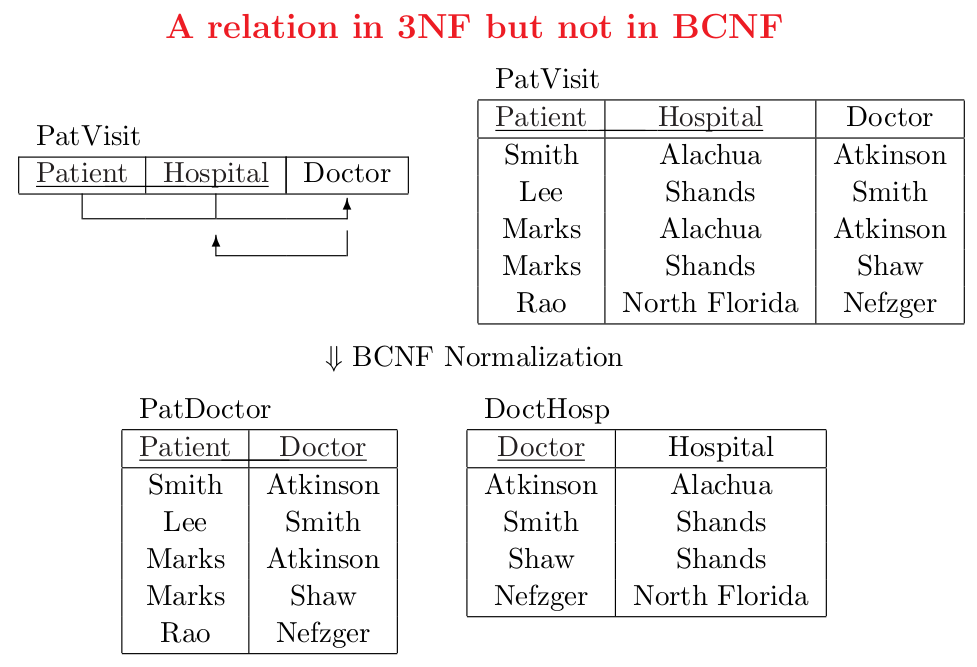
\includegraphics[width=.5\textwidth]{fig/bcnf-contre.png}
\caption{Contre-Exemple de BCNF}
\end{figure}

\subsubsection{Quatrième forme normale}
\paragraph{Dépendance multivaluée} Une dépendance $X \rightarrow\rightarrow Y$
est multivaluée si on peut définir un ensemble de valeurs admissibles pour $Y$
pour $X$ connu.

Une dépendance multivaluée triviale est le cas particulier $(X \subseteq Y) \lor (X \cup Y = R)$.

\paragraph{Définition}
Une relation est en 4NF si elle est en 3NF et que pour chacune de ses
dépendances multivaluées non triviales $X \rightarrow\rightarrow Y$, $X$ est
une super-clef.

\subsubsection{Cinquième forme normale}
Une relation est en 5NF si elle est en 4NF et qu'il n'est plus possible de la
décomposer sans perte d'informations.


\end{document}
